\chapter{Background}

\section{Software engineering}

The craft of software engineering emerged during the 1960s. Software crisis, the growing gap between expectations and results for software, called for a more systematic approach to software production~\cite{naur_peter_software_1969}. Authors suggested that software should be considered a branch of engineering, like hardware. NATO-organized conference in 1968 widely launched the new, engineering-inspired approach to software production.

Even though the comparison to engineering was initially used to provoke thought~\cite{naur_peter_software_1969}, it has since become a part of the software production vocabulary. However, the concept of software engineering has remained a topic of dispute in academia. \citet{boehm_software_1979} leans to the Webster dictionary definitions for software and engineering, combining them to a formal definition of software engineering: applying science to create "useful to man" computer programs and documentation. He argues that the difference between arbitrary development and software engineering is that the latter ensures the result is useful for the end-users, satisfying the specification. On the other hand, Sommerville establishes the gap between software development and software engineering: he defines software development as the actual development process where code is written, whereas software engineering is tied to the life cycle of the software – from planning to maintenance.~\cite{sommerville_software_2016}

The engineering mindset and the lifecycle of the software are included in IEEE's take on software engineering. The definition can be described as combining Boehm's and Sommerville's definitions. For this thesis, we will be using the IEEE definition.~\cite{ieee_ieee_1990}

Software engineering can be divided into four main activities: software specification, development, validation, and evolution.~\cite{sommerville_software_2016} These steps can also be called a software process or a software development life cycle (SDLC). Commonly used SDLCs include the Waterfall model, Validation \& Verification model (V model), and Agile methods.~\cite{balaji_waterfall_2012} Projects can benefit from different approaches: dimensions such as level of risk, budget, or project timeline vary between the SDLCs.~\cite{alshamrani_comparison_2015, cohen_introduction_2004} The industry data shows a trend towards the iterative approaches~\cite{sommerville_software_2016}. 

\subsection{Waterfall model}

The so-called Waterfall model is widely referred to as the most well-known SDLC. Waterfall model consists of 5 sequential process stages: requirements analysis, design, coding, testing, and maintenance.~\cite{alshamrani_comparison_2015} As the name implies, a project following the Waterfall model is one-way: it moves only forwards, and the different stages do not overlap. Each stage produces a deliverable to be used as a basis for the upcoming stage~\cite{balaji_waterfall_2012}. 

In practice, projects rarely blindly follow the Waterfall model: upcoming stages are prepared parallel to the current one, and previous stages are revisited when the need arises.~\cite{sommerville_software_2016} This "iterative Waterfall" is in line with the original model from the research paper Waterfall is derived from: the author originally intended the method to be used in an iterative manner~\cite{royce_managing_1987}.

A major shortcoming of the Waterfall model is that the software is delivered only once. On the other hand, it is good if the requirements are well-known beforehand and stay relatively static during the project. For example, a security system for a power plant would be a potential use case for the method.

\subsection{Agile methods}

Agile methods is an umbrella term that includes methodologies like Extreme Programming~\cite{wells_don_extreme_2018}, Lean Development, and Scrum~\cite{scrumorg_home_2022}. The terminology is further complicated due to the improper usage of the term in the industry. The common properties of Agile methods include iterative development, focus on communication, and a critical stance toward intermediate deliverables like requirements. Furthermore, Agile evangelists have agreed that Agile is more about a "state of mind" rather than a single process or methodology.~\cite{cohen_introduction_2004}

In iterative development, new versions of a working product are delivered constantly: most productive teams deploy software to production even multiple times in a day~\cite{forsgren_accelerate_2018}. This approach enables the end-users to use the software from the early days of the development cycle. Development teams can receive constant feedback from users and iterate the software accordingly for the next releases.~\cite{balaji_waterfall_2012}

Focus on communication encourages development teams to enable low-threshold, constant communication practices instead of documentation-heavy decision-making methods. Agile methods introduce practices like daily stand-up meetings and pair programming to support this~\cite{fowler_agile_2001}. When Agile methods emerged, co-locating team members were also seen as the key to success for working communication~\cite{cohen_introduction_2004}. With the possibilities presented by modern collaboration platforms like Slack and Zoom, low threshold communication has become possible for remote teams – working from the same physical location is no longer seen as crucial for Agile implementation.

Another definitive characteristic of Agile methods is the critical stance toward intermediate, non-critical deliverables. By reducing the resources spent on these artifacts, teams can focus their efforts on developing the product.~\cite{cohen_introduction_2004} The self-managing nature of Agile teams further promotes the idea that they have the best context to prioritize and plan their work.~\cite{alshamrani_comparison_2015} 

Even though Agile has an evergrowing status in the software development world, traditional methods like Waterfall are still needed. Large teams and complex projects are seen as environments where more structured processes should be preferred. On the other hand, teams are increasingly incorporating Agile properties into their traditional software processes and vice versa.~\cite{cohen_introduction_2004} 

\subsection{DevOps}

Agile has transformed the way software is developed. However, in the software lifecycle, the performance of testing, deployment, and post-deployment functions like fault recovery should be considered. DevOps brings development and IT operations closer together, bridging the gap between these silos and enabling responsiveness throughout the lifecycle of the software~\cite{hemon-hildgen_agile_2020}. DevOps aims to shorten the software development lifecycle by introducing automated tools that ship code to production faster, boosting both productivity and quality of development\cite{cois_modern_2014}. According to~\citet{humble_why_2011}, DevOps practices can be divided into four main aspects: automation, culture, sharing, and measurement. 

The most distinctive automation practices introduced by DevOps are continuous integration (CI) and continuous delivery (CD). In continuous integration, the developers' changes are often submitted back to the main branch as soon as possible, usually preceded by a build task and automated unit tests run by a CI worker. CI is often followed by CD, which is in charge of integration testing, end-to-end testing, and finally, deploying the approved version into a staging environment. The abbreviation "CD" is commonly also used to refer to continuous deployment. 

In addition to the steps in continuous delivery, continuous deployment automates software deployment to production environments. In contrast, continuous delivery pipelines require the user's manual interaction to initialize deployments. In the industry, CD usually refers to continuous delivery, though the term is used in quite a liberal manner. Systems consisting of both CI and CD functions are called the CI/CD pipeline. In modern-day DevOps, a stable CI/CD pipeline is the backbone of the team's success: In addition to customer satisfaction, implementing these practices can have an organizational impact, such as improved work satisfaction \cite{forsgren_accelerate_2018}. 
 
In essence, DevOps is about ways of working. Sociotechnical factors must be considered to create a well-functioning DevOps function~\cite{hemon-hildgen_agile_2020}. Implementing DevOps requires changes to the organization's work culture and a change of mindset from individual contributors. For example, rotating responsibilities and increased information sharing are ways to enforce DevOps practices.~\cite{lassenius_agile_2015}

Measuring processes is a cornerstone of increasing efficiency. In DevOps, production environments are measured continuously, and these metrics are used as gauges of development productivity~\cite{lassenius_agile_2015}. An increasing trend is also to measure the development processes directly: For example, statistics from version control systems are analyzed to extract information on the organization's health~\cite{forsgren_accelerate_2018}.

\section{Developer productivity}

\subsection{Productivity in general}
Productivity in industrial engineering is defined as the ratio of input and output\cite{syverson_what_2011, chew_no-nonsense_1988}. In manufacturing, input and output are relatively easily measured as the used resources and the produced goods. On the other hand, non-manufacturing businesses rely on more complex definitions: in knowledge work, person-hour is not considered a relevant metric of productivity~\cite{tangen_demystifying_2005}. The definition of output has also been under debate. In 1988, Chew proposed that output should include metrics other than "the number of units," for example, quality, timeliness, and price of the product~\cite{chew_no-nonsense_1988}. Many relatively similar context definitions have also emerged in the literature~\cite{tangen_demystifying_2005}.

The terms productivity and performance are sometimes used interchangeably. To further complicate the terminology, the authors define performance as a component of productivity and vice versa. Based on a vast amount of literature research, Tangen defines performance as an "umbrella term of excellence" consisting of productivity and other non-cost elements. In contrast, productivity is defined as a "physical phenomenon" – the ratio of input and output~\cite{tangen_demystifying_2005}. As an example of the opposite approach, SPACE authors define performance as the "outcome of a system or process," measured by metrics like service health or customer satisfaction. Productivity in the SPACE framework is about the sum of its parts, with performance as one of them~\cite{forsgren_space_2021}. To sum things up, these terms are used to refer to varying phenomena in different situations.

In the examples before, productivity is reviewed from the company's perspective. Often it is beneficial to look into the metrics of a smaller entity: a department, a team, or an individual~\cite{forsgren_space_2021, tangen_demystifying_2005}. These metrics can provide more accurate insights into the entity in question.

When measuring the productivity of teams or individual employees, it can be tempting to incentivize them based on the metrics. For example, software developers could get promotions or raise if they contribute more than average to the product. Often these ambitions can lead to unwanted results as employees optimize their work to meet the metric rather than focusing on the company's interests~\cite{symons_software_2010, chew_no-nonsense_1988}. For example, if the metric used was the number of pull requests, it would be tempting to break the work into tiny increments to pump up the numbers. Individual preferences further tricky the topic, as some employees by habit contribute more commits than others~\cite{oliveira_code_2020}. 

\subsection{Productivity in software engineering}
Determining the productivity of engineers is seen as crucial for the success of software development. Therefore, substantial research has been conducted in the past years.\cite{oliveira_code_2020} No consensus has been found on measuring productivity accurately. Historically, source code-based metrics such as lines of code or amount of commits have been utilized~\cite{oliveira_code_2020}. Nowadays, these metrics are considered, at best, an incomplete representation of the true productivity~\cite{forsgren_space_2021}.

Modern frameworks have explored the work of a software engineering team as a joint effort: as popular SDLCs emphasized teamwork, productivity should be assessed in the same context. The team is seen as the "basic work unit"~\cite{moe_overcoming_2010}, and the research has shifted towards how teams can improve together. Even though high-performing individuals are still seen as a valuable asset, companies should focus on building and enabling high-performing teams~\cite{forsgren_space_2021}. 

Agile methods estimate productivity by estimating velocity – units of completed work in a time frame. Although velocity is considered a better indicator of productivity than source code metrics, it has significant drawbacks. The topic is widely covered by \citet{forsgren_accelerate_2018} in their industry-shaping book \textit{Accelerate: The Science of Lean Software and DevOps: Building and Scaling High Performing Technology Organizations}. Most importantly, velocity is highly relative to the context and should not be used as an absolute metric. Secondly, velocity is an excellent example of a metric prone to be gamed by the employees, as described previously.~\cite{forsgren_accelerate_2018}
 
\subsection{Developer productivity frameworks}

Partly due to the misconceptions about developer productivity, research has gravitated towards finding reliable ways to discuss, measure, and enhance developer productivity. DevOps Research and Assessment (DORA), an Alphabet Inc subsidiary, has pioneered the research of DevOps and developer productivity. In their book Accelerate, they present four key metrics to measure software delivery performance, often referred to as the DORA metrics. The metrics are as follows: 

\begin{enumerate}
\item Lead Time
\item Deployment Frequency
\item Mean Time to Restore
\item Change Fail Percentage
\end{enumerate}

Lead Time is a metric derived from Lean manufacturing to the software context. It refers to the time from a feature request to the change that fulfills the request. Often in software, the changes are not directly requested by single customers but instead decided by the teams using large amount of input from stakeholders. DORA metrics define Lead Time as the time from the first commit to code running in the production environment~\cite{forsgren_accelerate_2018}.

In this thesis, we use Lead Time to refer to the time from the first commit to a new branch to the moment it is merged to the main branch, as seen in figure \ref{fig:CycleTime}. The industry term for this metric is Pull Request Cycle Time. 

\begin{figure}[ht]
    \begin{center}
        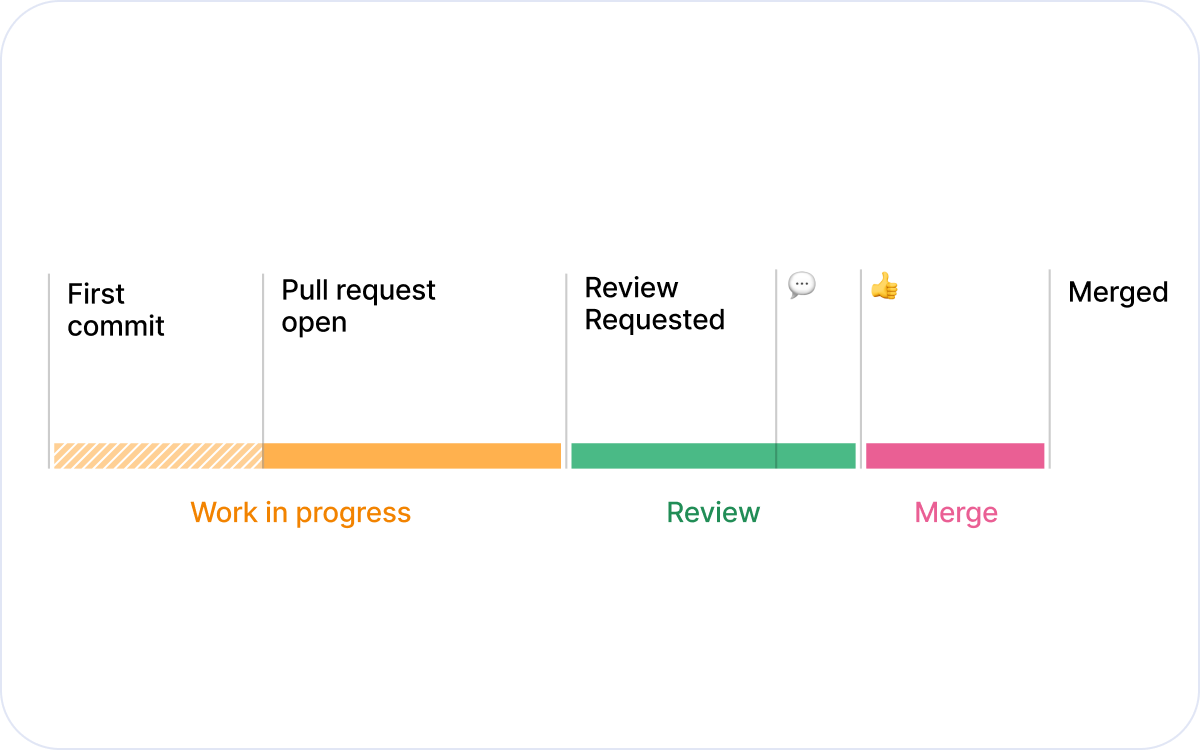
\includegraphics[width=13.5cm]{images/cycletime-defined}
        \caption{Pull Request lifecycle~\cite{swarmia_reducing_2022}}
        \label{fig:CycleTime}
    \end{center}
\end{figure}

Batch size has been popularized by it's use as a key performance metric in the Toyota Production System~\cite{ono_toyota_1988}. DORA researchers note that batch size is a sub-optimal metric in the software development context. Therefore, they chose Deployment Frequency as a suitable proxy to estimate the batch size. Deployment Frequency is the frequency of pushing a new version to the production environment.  

Lead Time and Deployment Frequency are metrics for software delivery tempo. Two additional metrics are used to determine if the increase in tempo has disadvantages in terms of software quality or system stability: Mean Time to Restore and Change Fail Percentage. Both of these measure situations where the production environment has failed. The authors articulate that failure is a common situation in rapidly changing software systems, and the absolute amount of failures is an obsolete metric. Instead, they propose two better suitable metrics: the time used to restore an application after an incident and the percentage of changes that lead to a production system failure. 

In Accelerate, the results are precise: increasing software delivery tempo has no negative impact on stability or quality. Instead, teams that performed well in the first two metrics also had better results in the rest measures. 

A more recent work from the DORA team is called the SPACE framework. The framework is named after its dimensions: satisfaction and well-being; performance; activity; communication and collaboration; and efficiency and flow. The framework extends DORA metrics by including, for example, perceived metrics. 

The researchers argue that productivity measurement should not rely on a single metric but rather include at least three metrics from the SPACE dimensions. Furthermore, the metrics should include quantitative, qualitative, and individual and team-level metrics. Also, performance measures on the organizational level are critical to getting a comprehensive image of productivity. 

The SPACE publication proposes a set of example metrics to concretize the framework. These proposals are not to be used as is but rather serve as an inspiration for those developing productivity tracking systems.~\cite{forsgren_space_2021}

\section{Software engineering as teamwork}

Work is often organized around teams. To distinguish a team from other groups that work together, we use the definition by Katzenbach \& Smith: "a team is a small number of people with complementary skills who are committed to a common purpose, set of performance goals, and approach for which they hold themselves accountable"~\cite{katzenbach_discipline_1993}. The fundamental difference is the accountability on both individual and team levels: team members are primarily responsible for each other, their supervisors, or other stakeholders~\cite{katzenbach_discipline_1993}.

In software engineering, teams work together to design, develop and maintain products. Working as a team offers upsides such as increased employee satisfaction, innovation, and productivity~\cite{moe_teamwork_2010}. In modern software development, the team is considered as the basic work unit rather than the individual contributor~\cite{moe_overcoming_2010}. This shift has motivated companies and executives to focus on building hyper-performing teams.

\subsection{Self-managing teams}

Modern software development methods encourage, or even insist on, the use of self-mana\-ging teams~\cite{moe_teamwork_2010,fowler_agile_2001}. Other terms used to define the phenomena include self-organizing team, autonomous team, and empowered team. Even though most studies report that forming self-managing teams leads to positive outcomes, there have also been opposing conclusions. Factors like poor leadership or the broader nature of the situation can lead to the difficulty of implementing such a team~\cite{moe_teamwork_2010}. 

To enable genuine self-management within a team, company leadership and other internal stakeholders must respect the team's independence and improvement efforts~\cite{moe_overcoming_2010}. Additionally, teams are not usually designated with a leader: instead, they are expected to form processes for a shared leadership function. Even though shared leadership can lead to better functioning teams, it adds more complexity and requires better cohesion and communication.~\cite{solansky_leadership_2008}

To improve, self-managing teams have to change their behavior, either by self-managing or from an external stimulus. Teams that can self-improve can achieve more autonomy than their counterparts. Norms, standards that regulate team members' behavior, are of the essence when building a productive software development team~\cite{abrahamsson_exploring_2016}. Norms can include technical and non-technical rules; for example, teams can commit to test-driven development or promote pair programming. The impact of norms for development teams is achieved through increased simplicity of standard processes: team members can trust that their colleagues do certain activities and refrain from the unwanted ones~\cite{abrahamsson_exploring_2016}. 

Team norms can be formed in two ways: organically within the team or by others, or as part of the organization's guidelines or direct influence~\cite{teh_social_2012}. Agile teams tune their ways of working during sprint retrospective meetings. Teams can also host dedicated sessions to discuss their norms: many SDLCs encourage teams to review their methods regularly. To enforce the norms, teams use whiteboards, notifications, and other reminders to refresh their memory and keep each other accountable.  

\subsection{Tools for teamwork}

Teams use a large number of tools to facilitate their work. Issue trackers like Jira, version control systems like Git, and chat tools like Slack play a central role in the day-to-day interaction of software development teams. Many team norms revolve around how team members are expected to use these applications. For example, the developers could commit to preferring public channels over direct messages in an instant messaging program.

 As a large part of information-intensive work is done using IT systems, there lies a remarkable efficiency improvement potential in these tools. Teams can aim to boost their performance with the help of software. For example, using web-based spreadsheet editor can reduce the need for manually sharing new versions within the team.

In addition to systems designed to help teams work together, there exists software solutions to improve team performance. Especially in software development, where the team's outputs are mainly lines of code, it is a tempting idea to conduct team performance metrics from the codebase~\cite{mcintosh_empirical_2016}. Authors argue that these kind of tools are problematic, as they only focus on outputs, reduce quality out of the equation and in essence, provide a one-sided view on the team's health~\cite{forsgren_space_2021, forsgren_accelerate_2018, oliveira_code_2020}.

To tackle this dilemma, a new wave of solutions addressing team performance has emerged. The tools are openly opinionated and aim to influence their client companies to use specific popular development methodologies, such as Continuous Integration. Examples of such tools include LinearB~\cite{linearb_developer_2022}, Haystack~\cite{haystack_haystack_2022}, Jellyfish~\cite{jellyfish_align_2022}, and Swarmia~\cite{swarmia_gain_2022}. Even though these tools utilize version control as input for their insights, they aim to offer a multi-sided, research-backed metrics for the teams.

\section{Managing change}

Change management is a systematic approach for organizational change. The change itself is an evident element of all organizations: planned change on the other hand requires direct efforts from the company. A vast number of change management frameworks have been proposed, with no single solution for all situations found.~\cite{todnem_organisational_2005}

\subsection{Making change stick}

It has been generally proven that to make users conform to change, the new changes should be in line with their team's norms~\cite{terry_attitude-behaviour_2000}. Therefore, organizations should look into current norms and enforce changes in them while introducing broader organizational change. Without this step, things might change on the surface, but no actual change is achieved. 

The stronger individuals identify with their team, the stronger the group opinion's effect is: the individuals tend to align with the group's view on the norms \cite{terry_attitude-behaviour_2000}. High cohesion is usually a positive phenomenon, but this situation can cause conflict with the organization's change initiatives. Instead of winning the individuals over one by one, it is also necessary to change the team's collective views.

\citet{kotter_leading_1995} summarizes that by making change stick, people will not revert to their old ways. Often, the change initiatives are handled as projects that are additional to the actual work. In a modern, constantly changing work environment, it is therefore important to focus on stickiness instead of short-term wins. The change must be woven into the day-to-day methods, making it a natural part of how teams work. On the other hand, short-term wins, such as achieving weekly goals, are an important way to motivate people for long-term change.~\cite{kotter_leading_1995}

\subsection{Individuals and change}

The role of individual contributors (ICs) is arguably significant in organizational change. In software development, the success of change can be concentrated into three significant factors: the engineers' knowledge of the change outcomes, their view on the need for change, and their contribution to the change process.~\cite{lenberg_initial_2017} 

To spread knowledge on the upcoming change, the organizations must first create a vision of the future after the change. With a shared vision, it is easier to move the whole organization into one common direction~\cite{kotter_leading_1995}. To achieve a shared view of the change, organizations must communicate it clearly, sharing knowledge throughout the organization. 

To initiate the need for change within individuals, it is necessary to create a sense of urgency: the change has to happen now, not in the future~\cite{lenberg_initial_2017}. Furthermore, the employees need to see the change as applicable and achievable~\cite{kotter_leading_1995}. In the end, employees have to be ready to compromise in the moment of change, which requires internal motivation for it~\cite{rehman_psychology_2021}. 

In self-managing teams, the lack of contribution is not a problem, as the team members make the decisions in the first place. When discussing change initiatives that emerge within the team, the contribution is in-built into the process. Of course, teams must ensure that all team members get a say in the matter. The change initiatives that start from an external stimulus, such as an organization-wide move to Agile, are the ones that require elaborate inclusion of the individual contributors. 

\subsection{Change in software development}

Software development best practices are constantly changing, requiring engineers to stay adaptive throughout their careers. As people move between organizations, they bring in new ways of working. This creates pressure for the teams to be able to digest the new methods and push the incoming employees to align with the current ones. 

Furthermore, software development is an industry with constantly changing requirements. This is one of the key reasons why methodologies like Agile have become so popular: they claim to help organizations cope with the vast amount of instability in the ever-changing business environment~\cite{hamed_popular_2013}. The improved internal processes are seen as a way to improve the product, for example, by reducing the errors in production~\cite{cugola_software_1998}.






